\chapter{Network Configuration}
\label{chap:network_configuration}
The network used for this experiment is a made by docker containers, 
which simulates a Local Area Network (LAN) with multiple hosts.
The network is composed by 6 containers, 
which are intentionally vulnerable. 
The Greenbone/OpenVAS tool is shipped as a OVA virtual machine,
used in virtualbox, which is connected to the same network of the containers,
so that it can scan them and identify their vulnerabilities.

\begin{figure}[h!]
    \label{fig:net-conf}
    \centering
    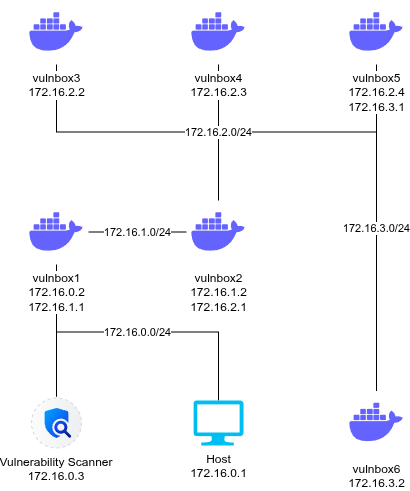
\includegraphics[width=0.8\textwidth]{../project/container-network.png}
    \caption{Network configuration}
\end{figure}